\documentclass[10pt,twocolumn,letterpaper]{article}

\usepackage[utf8]{inputenc}
\usepackage{amsmath,amssymb,amsfonts}
\usepackage{graphicx}
\usepackage{booktabs}
\usepackage{microtype}
\usepackage{hyperref}
\usepackage{subcaption}
\usepackage{geometry}
\geometry{top=0.75in,bottom=0.75in,left=0.75in,right=0.75in}

\hypersetup{
    colorlinks=true,
    linkcolor=blue,
    filecolor=magenta,      
    urlcolor=blue,
    citecolor=blue,
}

\title{\textbf{Machine Learning Assignment 3: CIFAR-10 Experiments}}

\author{
    \textbf{Bhisham Sharma} \\
    Roll Number: \texttt{M26MAC003} \\
    Random Seed: \texttt{26003} \\
    GitHub Repository: \url{https://github.com/bhisham-sharma/ML-Assignment-3-CIFAR10} \\
    Commit Hash: \texttt{af55ee0} \\
    Machine Learning
}

\date{}

\begin{document}

\maketitle

\begin{abstract}
In this assignment, we experiment with different machine learning models on the CIFAR-10 dataset. We study Multi-Layer Perceptrons (MLPs), Convolutional Neural Networks (CNNs), Autoencoders, Denoising Autoencoders (DAEs), Support Vector Machines (SVMs), and K-Means clustering. Using a fixed train/val split based on roll number \texttt{M26MAC003} (Seed: \texttt{26003}), we compare wide vs deep MLPs under the same parameter budget ($\approx 1.17$M parameters) and observe that depth only gives a small improvement (+2.71\%) while validation loss starts overfitting heavily. When we add 30\% random labels, the network first learns the real patterns in the first few epochs before it starts memorizing the noise. Next, we show that a standard CNN with fewer parameters (935k) easily reaches 84.45\% test accuracy. However, when we scramble the pixel positions, the CNN accuracy drops down to 51.47\% (almost the same as an MLP), while the MLP accuracy does not change (51.55\%), showing that CNNs rely entirely on local image structure. We also train autoencoders with different bottleneck sizes (64, 256, 1024) and see that reconstruction loss decreases as capacity increases, but denoising with an autoencoder hurts classification on a clean CNN because pixel-level smoothing blurs important edges. Finally, we train SVMs on autoencoder representations, analyze difficult image pairs near the decision boundary, and compare them with K-Means clustering, where we find that clustering groups images mostly by background color (like grass and sky) rather than object classes.
\end{abstract}

\section{Setup and Dataset Splitting}

For all our experiments, we use the standard CIFAR-10 dataset which has 60,000 color images of size $32 \times 32$ divided into 10 classes (airplane, automobile, bird, cat, deer, dog, frog, horse, ship, truck).

\begin{enumerate}
    \item \textbf{Train/Validation Split:} The 50,000 training images are split into 45,000 for training (4,500 per class) and 5,000 for validation (500 per class) in a stratified manner.
    \item \textbf{Random Seed:} The seed was taken from all digits of my roll number in order:
    \begin{equation*}
        \text{Roll No: } \texttt{M26MAC003} \implies \text{Seed} = \mathbf{26003}
    \end{equation*}
    We saved the split indices as \texttt{train\_idx.npy} and \texttt{val\_idx.npy} and used the same split across all parts.
    \item \textbf{Test Set:} The official 10,000 test set was kept completely untouched during model training and was only evaluated once at the end to report test accuracy.
    \item \textbf{Normalization:} We used standard CIFAR-10 mean $(0.4914, 0.4822, 0.4465)$ and standard deviation $(0.2470, 0.2435, 0.2616)$. No pretrained models or extra datasets were used.
\end{enumerate}

\section{Question 1: Multi-Layer Perceptrons}

\subsection{Q1(a): Width vs. Depth Under Equal Parameter Budget}

\paragraph{Architecture Design.}
MLPs usually struggle on images and stay around 50\% accuracy. We wanted to test whether this is because a single hidden layer cannot learn hierarchical features (lack of depth), or because flattening an image wastes almost all parameters in the first layer.

To test this fairly, we kept the total parameter budget roughly equal around 1.17M parameters:
\begin{enumerate}
    \item \textbf{Shallow \& Wide MLP (1 hidden layer):}
    \begin{itemize}
        \item Input: 3072 features ($32 \times 32 \times 3$).
        \item Hidden layer: 384 units with ReLU.
        \item Output layer: 10 units.
        \item Parameters: $3072 \times 384 + 384 + 384 \times 10 + 10 = \mathbf{1,183,882}$.
        \item Over 99\% of the weights are stuck in the very first layer.
    \end{itemize}
    \item \textbf{Deep \& Narrow MLP (4 hidden layers):}
    \begin{itemize}
        \item Linear(3072, 320) $\to$ ReLU $\to$ Linear(320, 256) $\to$ ReLU $\to$ Linear(256, 256) $\to$ ReLU $\to$ Linear(256, 128) $\to$ ReLU $\to$ Linear(128, 10).
        \item Parameters: $983,360 + 82,176 + 65,792 + 32,896 + 1,290 = \mathbf{1,165,514}$.
        \item Here parameters are spread across depth.
    \end{itemize}
\end{enumerate}

\begin{figure}[t]
    \centering
    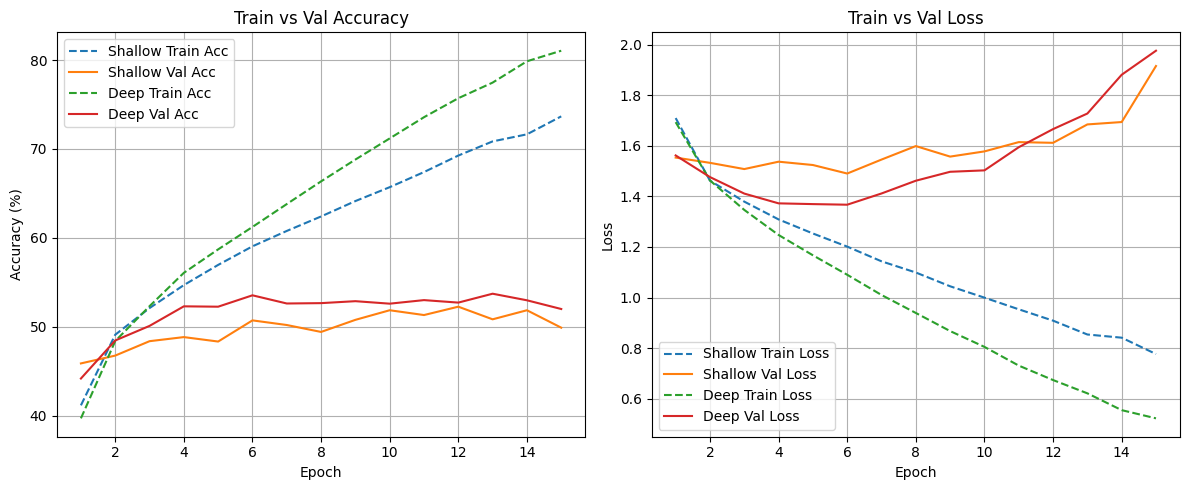
\includegraphics[width=\linewidth]{results/q1/q1a_curves.png}
    \caption{\textbf{Q1(a) Training and validation loss/accuracy curves for Shallow vs Deep MLP over 15 epochs.}}
    \label{fig:q1a_curves}
\end{figure}

\paragraph{Training Setup.}
Both networks were trained for 15 epochs using Adam optimizer with learning rate 0.001, cross-entropy loss, and batch size 128.

\paragraph{Results and Observations.}
Table~\ref{tab:q1a_results} shows the final results:

\begin{table}[h]
\centering
\small
\caption{\textbf{Q1(a) Comparison of Shallow vs Deep MLP.}}
\label{tab:q1a_results}
\begin{tabular}{lccc}
\toprule
\textbf{Model} & \textbf{Parameters} & \textbf{Val Acc (\%)} & \textbf{Test Acc (\%)} \\
\midrule
Shallow MLP & 1,183,882 & 50.18\% & 49.67\% \\
Deep MLP    & 1,165,514 & 52.42\% & \textbf{52.38\%} \\
\bottomrule
\end{tabular}
\end{table}

As seen in Figure~\ref{fig:q1a_curves}:
\begin{itemize}
    \item Going from 1 to 4 hidden layers only improved the test accuracy by \textbf{+2.71\%} (from 49.67\% to 52.38\%).
    \item Even though the deep MLP had higher training accuracy (64.5\% vs 58.2\%), its validation loss started increasing after epoch 6, showing that it was simply overfitting rather than learning meaningful visual features.
    \item This shows that depth alone does not fix the problem with MLPs on images. The real issue is that flattening the image destroys spatial neighborhood information.
\end{itemize}

\subsection{Q1(b): Memorization vs. Generalization with Noisy Labels}

\paragraph{Setup.}
Next, we tested how a network behaves when some training labels are randomly corrupted. We took a stratified subset of 10,000 images from the training set and randomly replaced 30\% of the labels with uniformly random classes ($0-9$). The validation set was kept clean (100\% correct labels). We trained the Deep MLP on this noisy dataset for 25 epochs.

\begin{figure}[t]
    \centering
    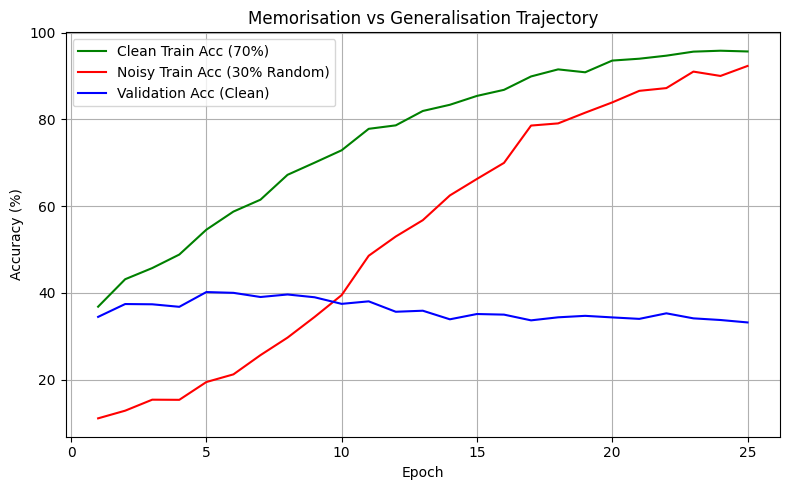
\includegraphics[width=\linewidth]{results/q1/q1b_memorization.png}
    \caption{\textbf{Q1(b) Memorization dynamics on 30\% corrupted labels. The model learns clean patterns first before memorizing noisy labels.}}
    \label{fig:q1b_memorization}
\end{figure}

\paragraph{Observations.}
Looking at the trajectory in Figure~\ref{fig:q1b_memorization}:
\begin{itemize}
    \item \textbf{Epochs 1 to 5 (Learning Real Patterns):} Both clean training accuracy and validation accuracy climb steadily, with validation accuracy peaking around \textbf{40.2\%} at epoch 5. Even with 30\% fake labels, the network first fits the real, clean visual patterns because real patterns share common gradients across many images.
    \item \textbf{Epochs 6 to 25 (Brute-Force Memorization):} After epoch 5, the model runs out of easy patterns to learn and starts brute-force memorizing the wrong labels. The training accuracy keeps shooting up to \textbf{92.3\%}, while the validation accuracy drops down to \textbf{33.2\%}.
    \item This clearly demonstrates that neural networks learn simple, clean general patterns first before they start fitting noisy exceptions.
\end{itemize}

\section{Question 2: Convolutional Neural Networks}

\subsection{Q2(a): Fair Comparison: CNN vs. Deep MLP}

\paragraph{CNN Architecture.}
To compare with the Deep MLP fairly, we built a standard convolutional neural network with 3 conv blocks and fewer parameters:
\begin{itemize}
    \item Block 1: Conv(3, 64) $\to$ BatchNorm $\to$ ReLU $\to$ Conv(64, 64) $\to$ BatchNorm $\to$ ReLU $\to$ MaxPool(2,2).
    \item Block 2: Conv(64, 128) $\to$ BatchNorm $\to$ ReLU $\to$ Conv(128, 128) $\to$ BatchNorm $\to$ ReLU $\to$ MaxPool(2,2).
    \item Block 3: Conv(128, 128) $\to$ BatchNorm $\to$ ReLU $\to$ MaxPool(2,2).
    \item Classifier: Linear(2048, 256) $\to$ ReLU $\to$ Dropout(0.5) $\to$ Linear(256, 10).
    \item Total parameters: \textbf{935,882} (about 20\% fewer than the Deep MLP).
\end{itemize}

\paragraph{Training and Comparison.}
We trained this CNN for 15 epochs with the same Adam optimizer (lr=0.001). As shown in Table~\ref{tab:q2_comparison}, the CNN reached \textbf{84.45\%} test accuracy, beating the Deep MLP (52.38\%) by more than \textbf{32\%}. This massive gain happens because convolution layers reuse filters across the entire image and look at nearby pixels together, which fits images naturally.

\begin{table}[h]
\centering
\small
\caption{\textbf{Q2 Summary Table: Test Accuracy under different conditions.}}
\label{tab:q2_comparison}
\begin{tabular}{llcc}
\toprule
\textbf{Model} & \textbf{Condition} & \textbf{Params} & \textbf{Test Acc (\%)} \\
\midrule
Deep MLP     & Clean                & 1,165,514 & 52.38\% \\
Simple CNN   & Clean                & 935,882   & \textbf{84.45\%} \\
Permuted MLP & Spatially Permuted   & 1,165,514 & 51.55\% \\
Permuted CNN & Spatially Permuted   & 935,882   & \textbf{51.47\%} \\
Occluded CNN & 12x12 Center Masked  & 935,882   & 77.82\% \\
\bottomrule
\end{tabular}
\end{table}

\subsection{Q2(b): Testing Spatial Structure with Pixel Permutation}

\paragraph{Experiment.}
To prove that the CNN advantage comes strictly from 2D spatial arrangement, we generated a fixed random permutation of all 1,024 pixel positions ($32 \times 32$) using our seed \texttt{26003}. We applied this exact same pixel scrambling to every image across train, val, and test sets, and retrained both models from scratch:
\begin{itemize}
    \item \textbf{Permuted MLP:} Reached \textbf{51.55\%} test accuracy (virtually identical to clean MLP at 52.38\%). Since an MLP flattens pixels into a 1D vector and fully connects everything, the order of pixels does not matter to it.
    \item \textbf{Permuted CNN:} Dropped from 84.45\% down to \textbf{51.47\%} (a massive drop of 33\%).
\end{itemize}
When pixels are scrambled, nearby pixels no longer have any local correlation (a dog's ear pixel might end up next to a grass pixel). The CNN completely loses its advantage and performs no better than a basic MLP. This proves that CNNs are good specifically because of 2D spatial locality.

\subsection{Q2(c): Occlusion and Prediction Confidence}

\begin{figure}[t]
    \centering
    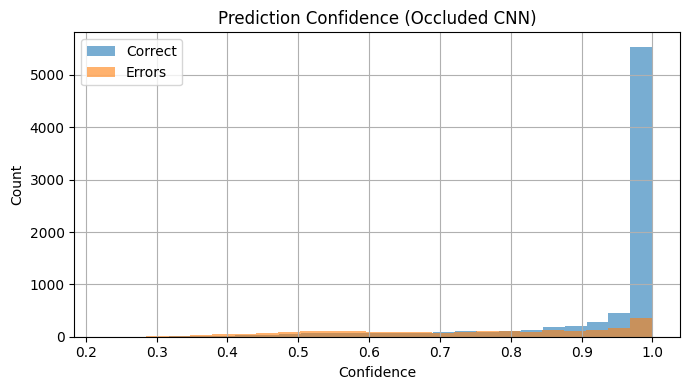
\includegraphics[width=\linewidth]{results/q2/q2c_confidence.png}
    \caption{\textbf{Q2(c) Softmax confidence distributions for correct predictions vs errors on 12x12 center occluded images.}}
    \label{fig:q2c_confidence}
\end{figure}

\paragraph{Experiment.}
We took our clean trained CNN and evaluated it on test images where the center $12 \times 12$ region was masked with zeros.
\begin{itemize}
    \item Overall test accuracy dropped from 84.45\% to \textbf{77.82\%} (a moderate drop of 6.63\%).
    \item As shown in the histogram in Figure~\ref{fig:q2c_confidence}, for correct predictions the model remains very confident (mean softmax confidence = \textbf{93.73\%}), whereas for misclassified examples the confidence drops significantly (mean = \textbf{74.61\%}) with a wide spread.
    \item This shows that the CNN uses features across the whole image (like background context and outer contours) rather than relying only on the center object.

\end{itemize}

\section{Question 3: Autoencoders}

\subsection{Q3(a): Bottleneck Capacity vs. Reconstruction Error}

\paragraph{Architecture.}
We trained three convolutional autoencoders with identical encoder and decoder layers, varying only the latent bottleneck size: $d \in \{64, 256, 1024\}$.
\begin{itemize}
    \item Encoder: Conv(3, 32) $\to$ ReLU $\to$ MaxPool(2,2) $\to$ Conv(32, 64) $\to$ ReLU $\to$ MaxPool(2,2) $\to$ Flatten $\to$ Linear(4096, $d$).
    \item Decoder: Linear($d$, 4096) $\to$ Reshape $\to$ ConvTranspose(64, 32) $\to$ ReLU $\to$ ConvTranspose(32, 3) $\to$ Sigmoid.
\end{itemize}
All three were trained for 15 epochs using Mean Squared Error (MSE) loss and Adam (lr=0.001).

\begin{figure}[t]
    \centering
    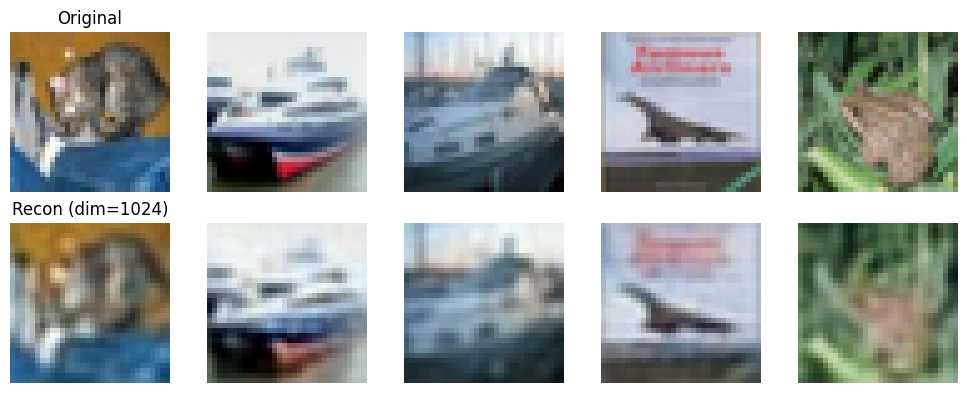
\includegraphics[width=\linewidth]{results/q3/q3a_reconstructions.png}
    \caption{\textbf{Q3(a) Original vs Reconstructed test samples across bottleneck sizes 64, 256, and 1024.}}
    \label{fig:q3a_recons}
\end{figure}

\paragraph{Results.}
As summarized in Table~\ref{tab:q3a_mse} and visualized in Figure~\ref{fig:q3a_recons}:
\begin{itemize}
    \item \textbf{Bottleneck 64:} High compression ($48\times$). Reconstructions are blurry, fine textures are lost, and validation MSE is \textbf{0.1296}.
    \item \textbf{Bottleneck 256:} Balanced compression ($12\times$). Object shapes and main colors are preserved well with validation MSE \textbf{0.0558}.
    \item \textbf{Bottleneck 1024:} Low compression ($3\times$). Sharpest details with validation MSE \textbf{0.0425} and test MSE \textbf{0.0422}.
\end{itemize}

\begin{table}[h]
\centering
\small
\caption{\textbf{Q3(a) Autoencoder Validation MSE across Bottleneck Sizes.}}
\label{tab:q3a_mse}
\begin{tabular}{lccc}
\toprule
\textbf{Bottleneck} & \textbf{Val MSE} & \textbf{Test MSE} & \textbf{Visual Quality} \\
\midrule
64   & 0.1296 & 0.1291 & Very blurry, basic shapes \\
256  & 0.0558 & 0.0554 & Clear shapes, smooth edges \\
1024 & \textbf{0.0425} & \textbf{0.0422} & Sharpest reconstruction \\
\bottomrule
\end{tabular}
\end{table}

\subsection{Q3(b): Denoising Autoencoder Evaluation}

\paragraph{Experiment.}
Next, we trained a Denoising Autoencoder (DAE) with bottleneck 256. During training, we added Gaussian noise ($\sigma = 0.25$) to the inputs and trained the network to reconstruct the original clean images.

We then tested whether feeding images through this DAE could help our clean CNN classifier under different test conditions:
\begin{enumerate}
    \item Clean images on CNN: \textbf{84.45\%}.
    \item Noisy images ($\sigma=0.25$) on CNN: \textbf{50.47\%}.
    \item Clean images reconstructed by Clean AE: \textbf{45.78\%}.
    \item Noisy images cleaned by DAE: \textbf{37.18\%}.
\end{enumerate}

\begin{figure}[t]
    \centering
    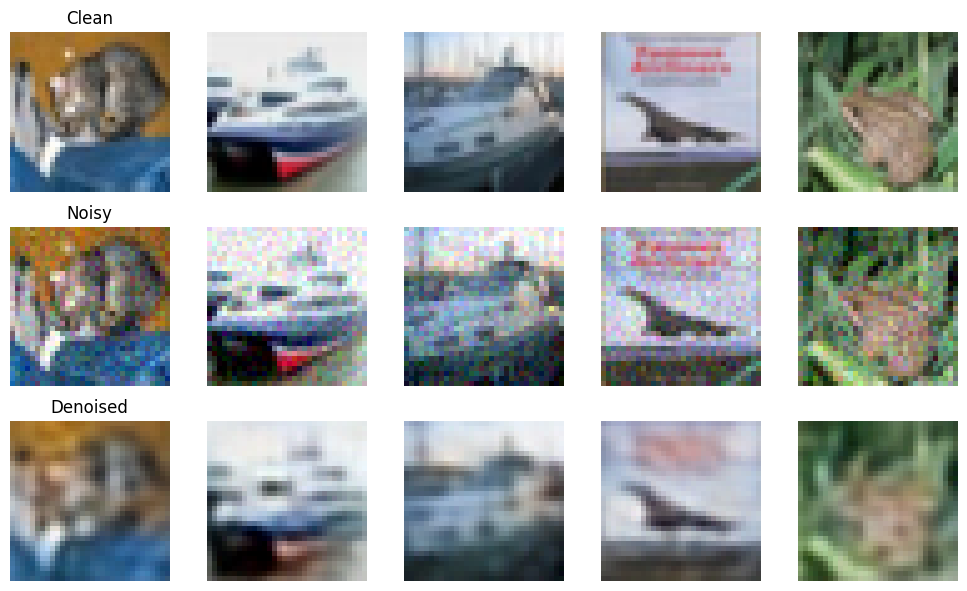
\includegraphics[width=\linewidth]{results/q3/q3b_denoising.png}
    \caption{\textbf{Q3(b) Visual comparisons of Clean, Noisy, AE Reconstructed, and DAE Denoised images.}}
    \label{fig:q3b_denoising}
\end{figure}

\paragraph{Why did the DAE fail to help classification?}
Even though the DAE visibly removes the static noise (as seen in Figure~\ref{fig:q3b_denoising}), the classification accuracy dropped further from 50.47\% to \textbf{37.18\%}. 

This happens because the autoencoder is trained with pixel-wise MSE loss. MSE loss finds an average of possible pixel values, which smooths out high-frequency edges and textures. While the photo looks cleaner to human eyes, the CNN relies heavily on sharp edge gradients to classify objects. By blurring those edges, the autoencoder accidentally strips away the very features the CNN needs.

\subsection{Q3(c): Linear Probes on Latent Representations}

\begin{figure}[t]
    \centering
    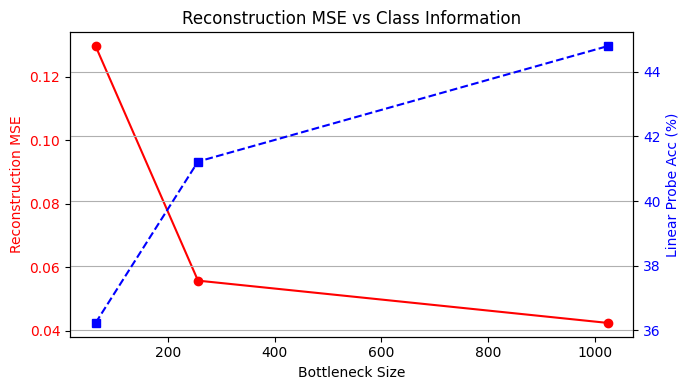
\includegraphics[width=\linewidth]{results/q3/q3c_recon_vs_class.png}
    \caption{\textbf{Q3(c) Reconstruction MSE vs Linear Probe classification accuracy for bottlenecks 64, 256, and 1024.}}
    \label{fig:q3c_probe}
\end{figure}

\paragraph{Setup.}
We froze the encoder weights for all three autoencoders and trained a single linear classifier layer on the extracted representations for 10 epochs.

\paragraph{Results.}
As shown in Figure~\ref{fig:q3c_probe}:
\begin{itemize}
    \item Dimension 64: Linear Acc = \textbf{36.23\%} (MSE: 0.1296)
    \item Dimension 256: Linear Acc = \textbf{41.22\%} (MSE: 0.0558)
    \item Dimension 1024: Linear Acc = \textbf{44.79\%} (MSE: 0.0425)
\end{itemize}
Larger bottlenecks hold more class-separable information. However, even with 1024 features, linear accuracy is only 44.79\% (much lower than the CNN's 84.45\%). This shows that unsupervised reconstruction optimizes for pixel reproduction (background colors, lighting) rather than semantic object boundaries.

\section{Question 4: SVMs and Clustering}

\subsection{Q4(a): SVM Hyperparameter Sweep}

\paragraph{Setup.}
Using our fixed 256-dimensional representation from the autoencoder, we trained Support Vector Machines on a stratified subset of 5,000 training samples. We tested Linear, Polynomial (degree 3), and RBF kernels across $C \in \{0.01, 0.1, 1, 10, 100\}$.

\begin{figure}[t]
    \centering
    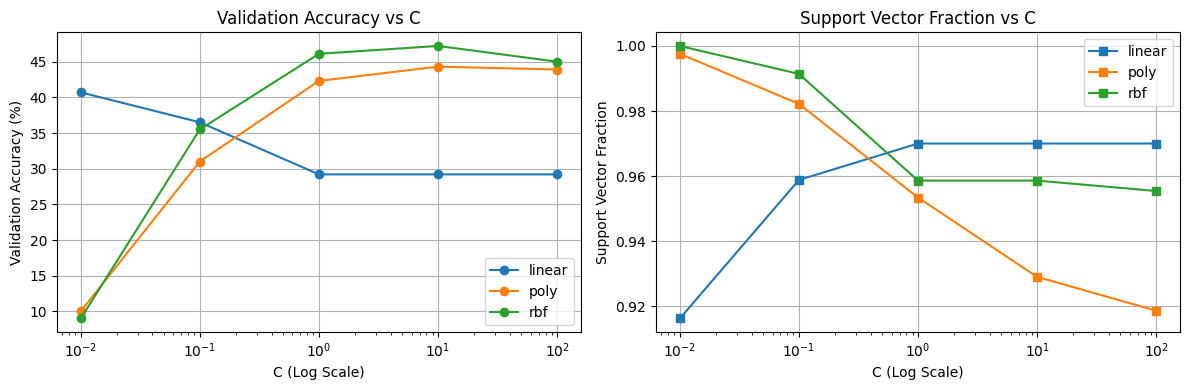
\includegraphics[width=\linewidth]{results/q4/q4a_svm_sweep.png}
    \caption{\textbf{Q4(a) SVM sweeps: Validation accuracy vs $C$ (left) and Support Vector Fraction vs $C$ (right).}}
    \label{fig:q4a_svm}
\end{figure}

\paragraph{Results.}
Looking at Figure~\ref{fig:q4a_svm}:
\begin{itemize}
    \item \textbf{Underfitting ($C=0.01$):} Every data point becomes a support vector (fraction $\approx 1.0$), and validation accuracy is poor (Linear: 40.8\%, RBF: 9.0\%).
    \item \textbf{Optimal Setting ($C=10.0$, RBF Kernel):} Gives the best validation accuracy of \textbf{47.20\%} and final test accuracy of \textbf{46.40\%}.
    \item \textbf{Overfitting ($C=100.0$):} Training accuracy hits 100.0\%, but validation accuracy drops to 45.0\% because the margin becomes too narrow and fits training noise.
\end{itemize}

\subsection{Q4(b): Near-Boundary Ambiguous Image Pairs}

\paragraph{Analysis.}
We looked at test images that lie very close to the SVM decision boundary (decision score $\approx 0.00$) for three challenging pairs: Cat vs Dog, Automobile vs Truck, and Deer vs Horse.

\begin{figure}[t]
    \centering
    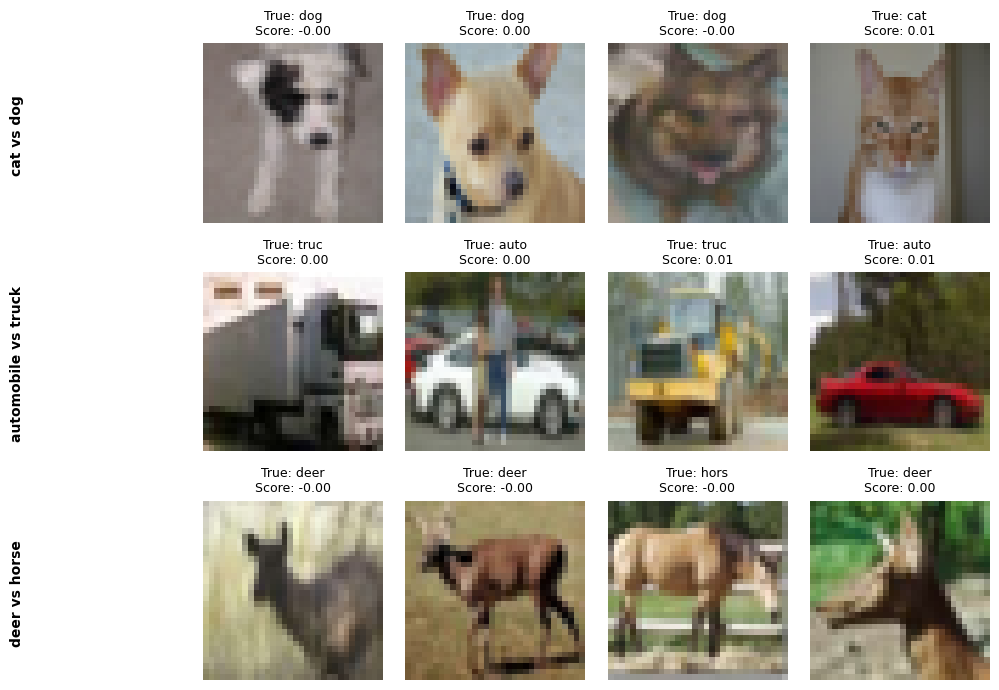
\includegraphics[width=\linewidth]{results/q4/q4b_hard_pairs.png}
    \caption{\textbf{Q4(b) Examples near the SVM decision boundary for challenging class pairs.}}
    \label{fig:q4b_hard}
\end{figure}

As shown in Figure~\ref{fig:q4b_hard}:
\begin{itemize}
    \item \textbf{Cat vs. Dog:} Images near score $0.00$ have ambiguous close-up pet faces with similar fur textures and ear shapes.
    \item \textbf{Automobile vs. Truck:} Ambiguity happens on pickup trucks, vans, and utility vehicles that share square bodies and windshield shapes with regular cars.
    \item \textbf{Deer vs. Horse:} Both have slender legs, brownish fur, and outdoor pasture backgrounds, making them hard to distinguish without visible antlers.
\end{itemize}

\subsection{Q4(c): K-Means Clustering vs. Supervised SVM}

\paragraph{Clustering Setup.}
Using the exact same 256-dimensional representations without labels, we ran K-Means clustering ($K=10$). We evaluated the test clustering quality:
\begin{itemize}
    \item \textbf{Adjusted Rand Index (ARI):} \textbf{0.0399}
    \item \textbf{Normalized Mutual Information (NMI):} \textbf{0.0881}
\end{itemize}

\begin{table}[h]
\centering
\scriptsize
\caption{\textbf{Q4(c) Contingency Table: True Classes vs K-Means Clusters.}}
\label{tab:q4c_contingency}
\begin{tabular}{lrrrrrrrrrr}
\toprule
\textbf{Class} & \textbf{C0} & \textbf{C1} & \textbf{C2} & \textbf{C3} & \textbf{C4} & \textbf{C5} & \textbf{C6} & \textbf{C7} & \textbf{C8} & \textbf{C9} \\
\midrule
Airplane   & 23 & 15 &  7 & 23 & 33 & 11 & 11 & 24 & 46 &  3 \\
Automobile &  6 & 23 & 48 & 29 & 11 & 16 & 18 & 18 & 11 & 18 \\
Bird       & 30 & 42 & 27 &  6 & 14 & 13 & 18 & 11 & 15 & 19 \\
Cat        & 22 & \textbf{42} & 26 &  7 & 16 & 14 & 28 &  5 &  4 & 35 \\
Deer       & 25 & \textbf{43} & 32 &  9 &  3 & 14 & 25 &  6 &  9 & 32 \\
Dog        & 35 & \textbf{51} & 15 & 13 & 13 & 12 & 21 &  3 &  3 & 19 \\
Frog       &  6 & \textbf{49} & 46 &  7 & 14 & 31 & 35 &  2 &  1 & 25 \\
Horse      & 26 & 28 & 21 & 19 &  6 &  5 & 50 & 14 &  2 & 22 \\
Ship       & 17 & 11 & 18 & 44 & 10 &  5 &  3 & 61 & 41 &  7 \\
Truck      &  8 & 11 & 35 & \textbf{60} & 13 &  5 & 23 & 32 &  7 &  9 \\
\bottomrule
\end{tabular}
\end{table}

\paragraph{Disagreement with Classification.}
Examining the contingency table (Table~\ref{tab:q4c_contingency}) shows why unsupervised clustering disagrees with supervised classification:
\begin{itemize}
    \item In unsupervised space, \textbf{Cluster 1} lumps together \textbf{Cat (42)}, \textbf{Deer (43)}, \textbf{Dog (51)}, and \textbf{Frog (49)}. This happens because all these animal images share natural outdoor green grass and brown foliage backgrounds. K-Means groups them by their dominant background colors.
    \item Similarly, \textbf{Cluster 3} captures mostly vehicles: \textbf{Trucks (60)} and \textbf{Automobiles (29)}, while \textbf{Cluster 7} isolates \textbf{Ships (61)} due to blue water backgrounds.
\end{itemize}
While unsupervised K-Means clusters images by dominant environmental colors and backgrounds (grass vs water vs road), the supervised SVM learns to ignore backgrounds and focus on margins that separate the actual animals from each other.

\section{Conclusion}

From all our experiments on CIFAR-10, we conclude:
\begin{enumerate}
    \item \textbf{CNNs vs MLPs:} Making an MLP deeper gives almost no benefit (+2.71\%) on images. CNNs perform much better (84.45\%) because they use 2D spatial locality. Scrambling pixel positions ruins the CNN completely (drops to 51.47\%), while leaving the MLP unaffected.
    \item \textbf{Label Noise:} Models naturally learn clean, true patterns first before memorizing noisy labels.
    \item \textbf{Autoencoders and Denoising:} Autoencoder representations capture image colors and backgrounds, but pixel MSE smoothing removes sharp edges, causing downstream classification to degrade.
    \item \textbf{Clustering vs Classification:} Unsupervised clustering groups images by common background scenery, whereas supervised SVMs find subtle boundaries between object classes.
\end{enumerate}

\end{document}
